\newpage
\subsection{Caso d'uso UC5: Gestione profilo utente}

\label{UC5}
\begin{figure}[ht]
	\centering
	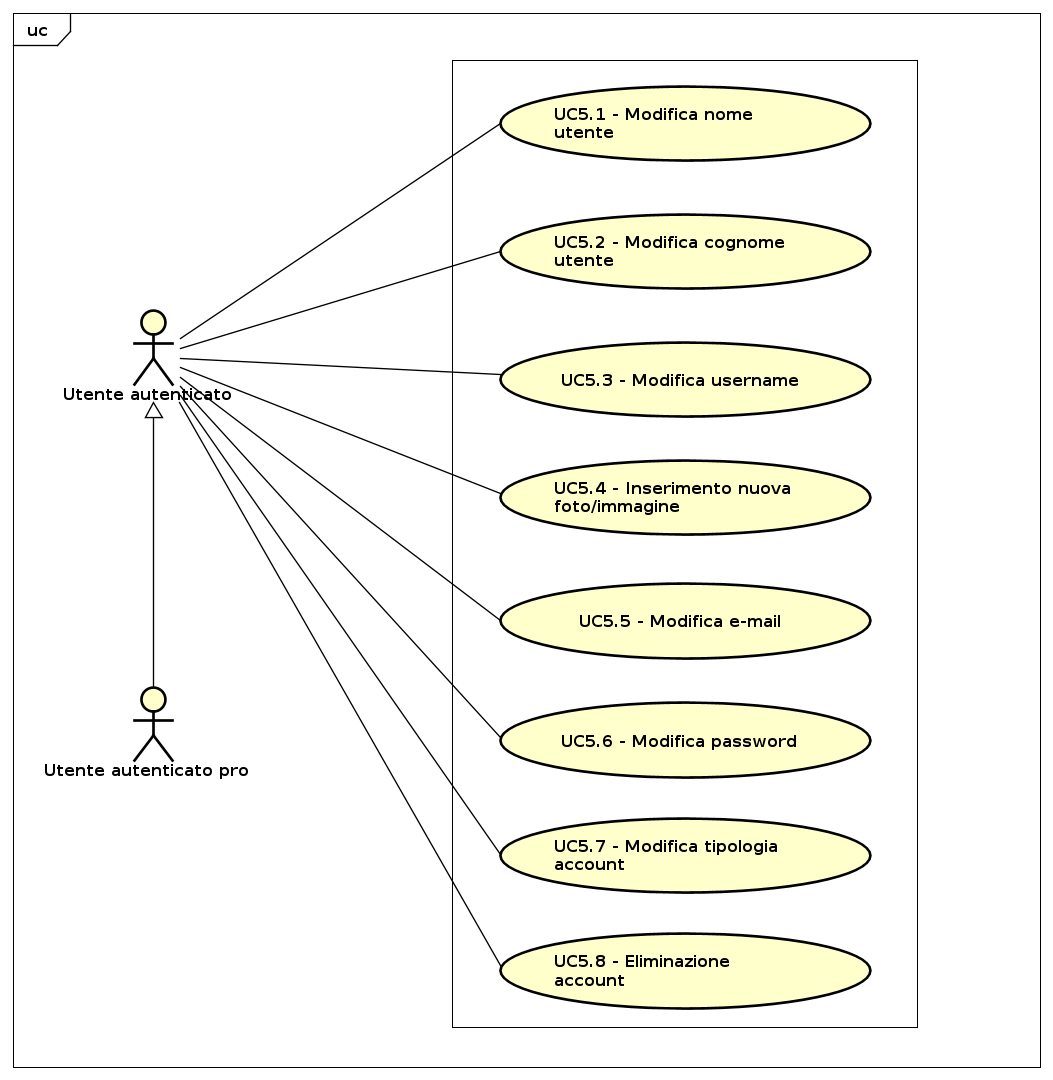
\includegraphics[scale=0.5,keepaspectratio]{UML/UC5.png}
	\caption{UC5: Gestione profilo utente}
\end{figure}
\FloatBarrier
\begin{itemize}
	\item \textbf{Attori}: utente autenticato, utente autenticato pro;
	\item \textbf{Descrizione}: l'attore può visualizzare e modificare i suoi dati personali;
	\item \textbf{Precondizione}: il sistema visualizza l'opzione di gestione profilo utente;
	\item \textbf{Postcondizione}: il sistema ha attuato le modifiche effettuate dall'attore ai propri dati personali;
	\item \textbf{Scenario principale}:
		\begin{enumerate}
			\item L'attore può modificare il proprio nome utente (UC5.1);
			\item L'attore può modificare il proprio cognome utente (UC5.2);
			\item L'attore può inserire una nuova foto/immagine per il proprio profilo utente (UC5.3);
			\item L'attore può modificare la propria e-mail (UC5.4);
			\item L'attore può modificare la propria password (UC5.5);
			\item L'attore può confermare le modifiche effettuate al proprio profilo utente (UC5.6)
			\item L'attore può modificare la tipologia del proprio account (UC5.8);
			\item L'attore può eliminare il proprio account (UC5.9).
		\end{enumerate} 
	\item \textbf{Estensioni}: l'attore visualizza un messaggio d'errore relativo alla conferma della modifica del profilo utente	(UC5.7);	 
\end{itemize}

\subsubsection{Caso d'uso UC5.1: Modifica nome utente}
\begin{itemize}
	\item \textbf{Attori}: utente autenticato, utente autenticato pro;
	\item \textbf{Descrizione}: l'attore può inserire un nuovo nome utente;
	\item \textbf{Precondizione}: il sistema visualizza l'opzione per l'inserimento nome utente;
	\item \textbf{Postcondizione}: l'attore ha inserito il nuovo nome utente;
	\item \textbf{Scenario principale}: l'attore inserisce il nuovo nome utente.
\end{itemize}

\subsubsection{Caso d'uso UC5.2: Modifica cognome utente}
\begin{itemize}
	\item \textbf{Attori}: utente autenticato, utente autenticato pro;
	\item \textbf{Descrizione}: l'attore può inserire un nuovo cognome utente;
	\item \textbf{Precondizione}: il sistema visualizza l'opzione per l'inserimento cognome utente; 
	\item \textbf{Postcondizione}:  l'attore ha inserito il nuovo cognome utente;
	\item \textbf{Scenario principale}: l'attore inserisce il nuovo cognome utente.
\end{itemize}

\subsubsection{Caso d'uso UC5.3: Inserimento foto/immagine}
\begin{itemize}
	\item \textbf{Attori}: utente autenticato, utente autenticato pro;
	\item \textbf{Descrizione}: l'attore può caricare una nuova foto/immagine;
	\item \textbf{Precondizione}: il sistema visualizza l'opzione per caricare una foto/immagine;  
	\item \textbf{Postcondizione}: l'attore ha caricato una nuova foto/immagine;
	\item \textbf{Scenario principale}: l'attore carica una nuova foto/immagine.
\end{itemize}

\subsubsection{Caso d'uso UC5.4: Modifica e-mail}
\begin{itemize}
	\item \textbf{Attori}: utente autenticato, utente autenticato pro;
	\item \textbf{Descrizione}: l'attore può inserire un nuovo indirizzo di posta elettronica;
	\item \textbf{Precondizione}: il sistema visualizza l'opzione per l'inserimento e-mail;
	\item \textbf{Postcondizione}: l'attore ha inserito un nuovo indirizzo di posta elettronica;
	\item \textbf{Scenario principale}: l'attore inserisce un nuovo indirizzo di posta elettronica.
\end{itemize}

\subsubsection{Caso d'uso UC5.5: Modifica password}
\label{UC5.5}
\begin{figure}[h]
	\centering
	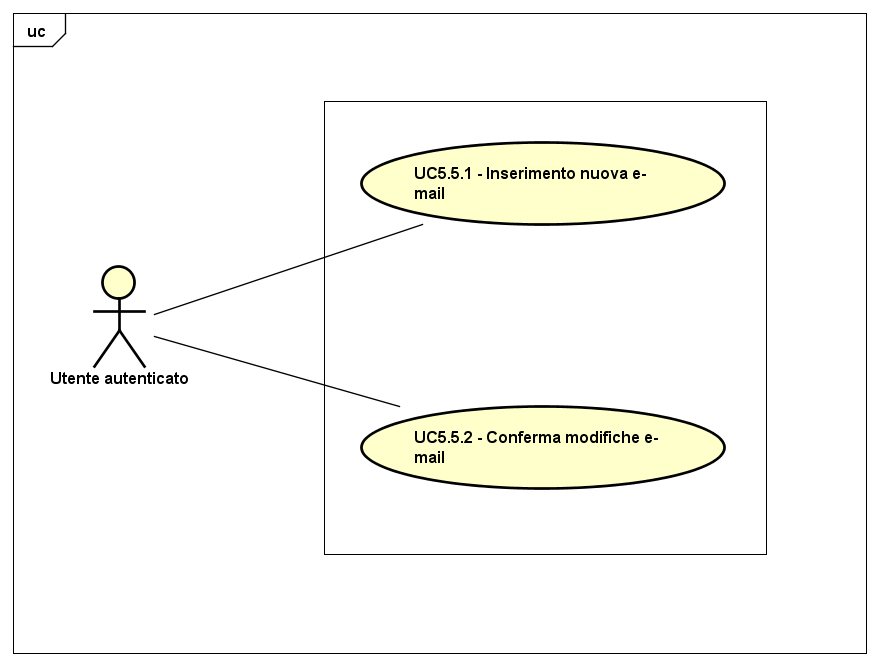
\includegraphics[scale=0.5,keepaspectratio]{UML/UC5_5.png}
	\caption{UC5.5: Modifica password}
\end{figure}

\begin{itemize}
	\item \textbf{Attori}: utente autenticato, utente autenticato pro;
	\item \textbf{Descrizione}: l'attore può modificare la propria password inserendone una nuova;
	\item \textbf{Precondizione}: il sistema visualizza l'opzione di modifica password;
	\item \textbf{Postcondizione}: il sistema ha reso persistenti le modifiche alla propria password;
	\item \textbf{Scenario principale}:
	\begin{enumerate}
		\item L'attore può inserire la propria vecchia password (UC5.5.1);
		\item L'attore può inserire una nuova password (UC5.5.2);
		\item L'attore può inserire la conferma della nuova password (UC5.5.3).
	\end{enumerate}
	\item \textbf{Scenari alternativi}: l'attore annulla le modifiche e il sistema lo riporta alla schermata di gestione del profilo utente.
\end{itemize}

\subsubsection{Caso d'uso UC5.5.1: Inserimento vecchia password}

\begin{itemize}
	\item \textbf{Attori}: utente autenticato, utente autenticato pro;
	\item \textbf{Descrizione}: l'attore può inserire la vecchia password;
	\item \textbf{Precondizione}: il sistema visualizza l'opzione per l'inserimento della vecchia password;
	\item \textbf{Postcondizione}: l'attore ha inserito la vecchia password;
	\item \textbf{Scenario principale}: l'attore inserisce la vecchia password.
\end{itemize}

\subsubsection{Caso d'uso UC5.5.2: Inserimento nuova password}

\begin{itemize}
	\item \textbf{Attori}: utente autenticato, utente autenticato pro;
	\item \textbf{Descrizione}: l'attore può inserire la nuova password;
	\item \textbf{Precondizione}: il sistema visualizza l'opzione per l'inserimento della nuova password;
	\item \textbf{Postcondizione}: l'attore inserisce la nuova password;
	\item \textbf{Scenario principale}: l'attore inserisce la nuova password.
\end{itemize}

\subsubsection{Caso d'uso UC5.5.3: Inserimento conferma nuova password}

\begin{itemize}
	\item \textbf{Attori}: utente autenticato, utente autenticato pro;
	\item \textbf{Descrizione}: l'attore può inserire la nuova password nuovamente;
	\item \textbf{Precondizione}: il sistema visualizza l'opzione per l'inserimento conferma nuova password;
	\item \textbf{Postcondizione}: l'attore inserisce nuovamente la nuova password;
	\item \textbf{Scenario principale}: l'attore inserisce nuovamente la nuova password.
\end{itemize}

\subsubsection{Caso d'uso UC5.6: Conferma modifiche profilo utente}

\begin{itemize}
	\item \textbf{Attori}: utente autenticato, utente autenticato pro;
	\item \textbf{Descrizione}: l'attore può confermare le modifiche apportare al proprio profilo utente; 
	\item \textbf{Precondizione}: il sistema visualizza l'opzione di conferma delle modifiche del profilo utente;
	\item \textbf{Postcondizione}: il sistema ha reso persistenti le modifiche al profilo utente;
	\item \textbf{Scenario principale}: l'attore conferma le modifiche apportate al proprio profilo utente;
	\item \textbf{Scenari alternativi}: l'attore annulla le modifiche e il sistema lo riporta alla schermata di gestione del profilo utente.
\end{itemize}

\subsubsection{Caso d'uso UC5.7: Visualizzazione errore conferma modifiche profilo utente}

\begin{itemize}
	\item \textbf{Attori}:  utente autenticato, utente autenticato pro;
	\item \textbf{Descrizione}: l'attore può visualizzare un messaggio d'errore se ha effettuato modifiche non permesse al proprio profilo utente;
	\item \textbf{Precondizione}: il sistema ha ricevuto dati vuoti o non validi;
	\item \textbf{Postcondizione}: il sistema mostra un messaggio d'errore;
	\item \textbf{Scenario principale}: l'attore visualizza un messaggio d'errore;
\end{itemize}

\subsubsection{Caso d'uso UC5.8: Richiesta cambio tipologia account}
\label{UC5.8}
\begin{figure}[h]
	\centering
	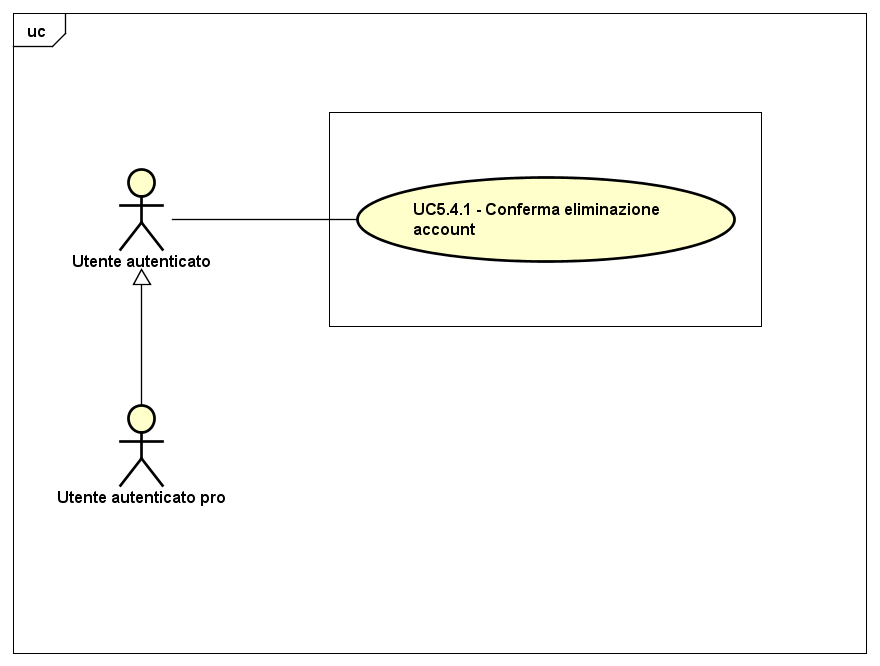
\includegraphics[scale=0.5,keepaspectratio]{UML/UC5_8.png}
	\caption{UC5.8: Richiesta cambio tipologia account}
\end{figure}

\begin{itemize}
	\item \textbf{Attori}: utente autenticato, utente autenticato pro;
	\item \textbf{Descrizione}: l'attore può richiedere di cambiare la tipologia del proprio account; 
	\item \textbf{Precondizione}: il sistema visualizza l'opzione di cambio tipologia utente;
	\item \textbf{Postcondizione}: il sistema invia la richiesta del cambio tipologia account;
	\item \textbf{Scenario principale}:
	\begin{enumerate}
		\item L'attore può selezionare il nuovo tipo di account a cui passare (UC5.8.1);
		\item L'attore può confermare l'invio della richiesta del cambio della tipologia del proprio account (UC5.8.2).
	\end{enumerate}
	\item \textbf{Scenari alternativi}: l'attore annulla le modifiche e il sistema lo riporta alla schermata di gestione del profilo utente.
\end{itemize}

\subsubsection{Caso d'uso UC5.8.1: Selezione tipologia account}

\begin{itemize}
	\item \textbf{Attori}: utente autenticato, utente autenticato pro;
	\item \textbf{Descrizione}: l'attore può selezionare una nuova tipologia di account a cui passare; se l'attore è un utente autenticato potrà scegliere di diventare un utente autenticato pro; se l'attore è un utente autenticato pro può scegliere di diventare un utente autenticato;
	\item \textbf{Precondizione}: il sistema visualizza le tipologie di account a cui passare;
	\item \textbf{Postcondizione}: l'attore ha selezionato  una nuova tipologia di account;
	\item \textbf{Scenario principale}: l'attore seleziona una tipologia di account a cui passare.
\end{itemize}

\subsubsection{Caso d'uso UC5.8.2: Invio richiesta cambio tipologia account}

\begin{itemize}
	\item \textbf{Attori}: utente autenticato, utente autenticato pro;
	\item \textbf{Descrizione}: l'attore può inviare la richiesta di passaggio alla nuova tipologia di account;
	\item \textbf{Precondizione}: il sistema visualizza l'opzione di invio richiesta cambio tipologia account;
	\item \textbf{Postcondizione}: il sistema invia la richiesta del cambio tipologia account;
	\item \textbf{Scenario principale}: l'attore invia la richiesta di cambio tipologia account.
\end{itemize}

\subsubsection{Caso d'uso UC5.9: Eliminazione account}
\label{UC5.9}
\begin{figure}[h]
	\centering
	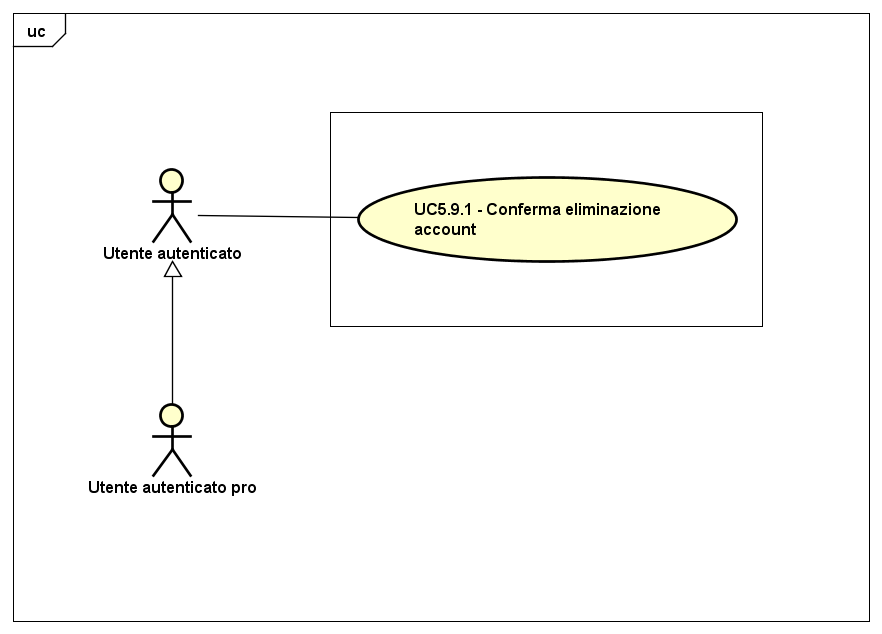
\includegraphics[scale=0.5,keepaspectratio]{UML/UC5_9.png}
	\caption{UC5.9: Eliminazione account}
\end{figure}

\begin{itemize}
	\item \textbf{Attori}: utente autenticato, utente autenticato pro;
	\item \textbf{Descrizione}: l'attore può eliminare il proprio account dal sistema; l'eliminazione dell'account comporta la cancellazione dei propri dati dal sistema; 
	\item \textbf{Precondizione}: il sistema visualizza l'opzione per l'eliminazione dell'account;
	\item \textbf{Postcondizione}: il sistema ha eliminato in maniera persistente l'account e tutti i relativi dati;
	\item \textbf{Scenario principale}: l'utente può confermare l'eliminazione del proprio account e dei relativi dati personali (UC5.9.1);
	\item \textbf{Scenari alternativi}: l'attore annulla l'eliminazione dell'account e il sistema lo riporta alla schermata di gestione del profilo utente.
\end{itemize}

\subsubsection{Caso d'uso UC5.9.1: Conferma eliminazione account}

\begin{itemize}
	\item \textbf{Attori}: utente autenticato, utente autenticato pro;
	\item \textbf{Descrizione}: l'attore può confermare la cancellazione del proprio account e dei relativi dati dal sistema;
	\item \textbf{Precondizione}: il sistema visualizza l'opzione per la conferma dell'eliminazione dell'account;
	\item \textbf{Postcondizione}: il sistema ha eliminato l'account dell'attore richiedente e tutti i relativi dati;
	\item \textbf{Scenario principale}: l'attore conferma l'eliminazione del proprio account.
\end{itemize}